\parindent=0em
\section{Tecnologías en realidad mixta}
\label{sec:oclusion}
\noindent

En la realidad mixta se hacen uso de las mismas tecnologías que las vistas en el apartado~\ref{techAR} de realidad aumentada. Aun así, para una correcta experiencia de realidad mixta es necesario también un buen efecto de oclusión.\\

La oclusión~\cite{oclussionExplanationEstadoDelArte}, ocurre cuando los objetos del mundo real están por delante de los objetos virtuales en la escena, si no hay oclusión, el objeto virtual se superpondrá al real creando la sensación de que el objeto real está detrás cuando realmente no es así (figura~\ref{fig:arcoreOclusionExample}).\\

Ya que en la realidad aumentada los objetos virtuales no tienen constancia de la existencia de los objetos del mundo físico, puede ocurrir que no haya una correcta oclusión entre elementos.\\

\begin{figure}[H]
\centering
    \hspace{-4mm}
    \begin{minipage}{0.5\textwidth}
        \centering
        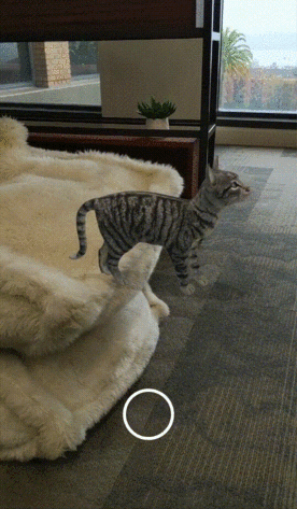
\includegraphics[scale=0.4]{Images/Estado del arte/nooclussion.jpg}\\
        (a) Realidad aumentada sin oclusión.
    \end{minipage}
    \begin{minipage}{0.5\textwidth}
        \centering
        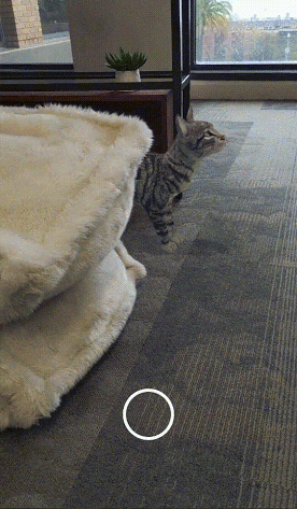
\includegraphics[scale=0.4]{Images/Estado del arte/sioclussion.jpg}\\
        (b) Realidad aumentada con oclusión.
    \end{minipage}\\
    \caption[Ejemplo del efecto de oclusión.]{Ejemplo del efecto de oclusión\footnotemark.}
    \label{fig:arcoreOclusionExample}
\end{figure}

\footnotetext{Fuente: \url{https://developers.googleblog.com/2019/12/blending-realities-with-arcore-depth-api.html}}
Para generar una buena oclusión en realidad aumentada, es necesario poder reconstruir el mundo real en 3D. Este es un proceso complicado ya que los dispositivos usados actualmente para AR no poseen los componentes necesarios para hacer esta reconstrucción de forma precisa y rápida, aun así, actualmente existen distintos métodos para generar oclusión~\cite{oclusionMethods}:

\begin{enumerate}
    \item \textbf{Mapa de profundidad}: En este caso se utiliza un sensor de profundidad para crear un mapa de profundidad en 2D (figura~\ref{fig:depthDiferido}), este mapa no es perfecto ya que hay huecos en él, asimismo, la resolución del mapa suele ser menor que la resolución de la cámara por lo que hay que escalar el mapa generando imperfecciones.
    
    \item \textbf{Mallas de oclusión}: En este método se crea una nube de puntos (apartado~\ref{sec:nubeDePuntos}) basados en la profundidad para posteriormente unir dichos puntos. De este modo, se crean mallas que reconstruyen el entorno en 3D y sirven como elemento para generar la oclusión.
\end{enumerate}

Ya que los dispositivos que se utilizan para AR (generalmente teléfonos móviles, de los que se habla en la sección~\ref{sec:telefonosMoviles}) generan una oclusión muy imprecisa en tiempo real con estos métodos, existen otros métodos para generar oclusión, pero en este caso, no se realiza la reconstrucción en tiempo real.\\



Por ejemplo, el estudio~\cite{oclusionEnDiferido} donde hacen una grabación del elemento sobre el que quieren generar la oclusión, aplican un algoritmo de visión por computador o visión artificial~\cite{visionporcomputador} (transformación de datos de una cámara a una nueva representación) para generar el mapa de profundidad explicado anteriormente. Este mapa generado (figura~\ref{fig:depthDiferido}) es muy preciso y de este modo se puede crear un efecto de oclusión sin grandes desajustes, todo esto utilizando únicamente una cámara monocular.\\

Por otro lado, si se conoce el entorno en el que se va a realizar la experiencia de realidad aumentada, se puede, previamente, recorrer el entorno repetidas veces generando una reconstrucción 3D del entorno más precisa que en tiempo real (generando una malla de oclusión). Posteriormente, esta reconstrucción se utiliza como modelo 3D para generar la oclusión.\\

\begin{figure}[H]
    \centering
    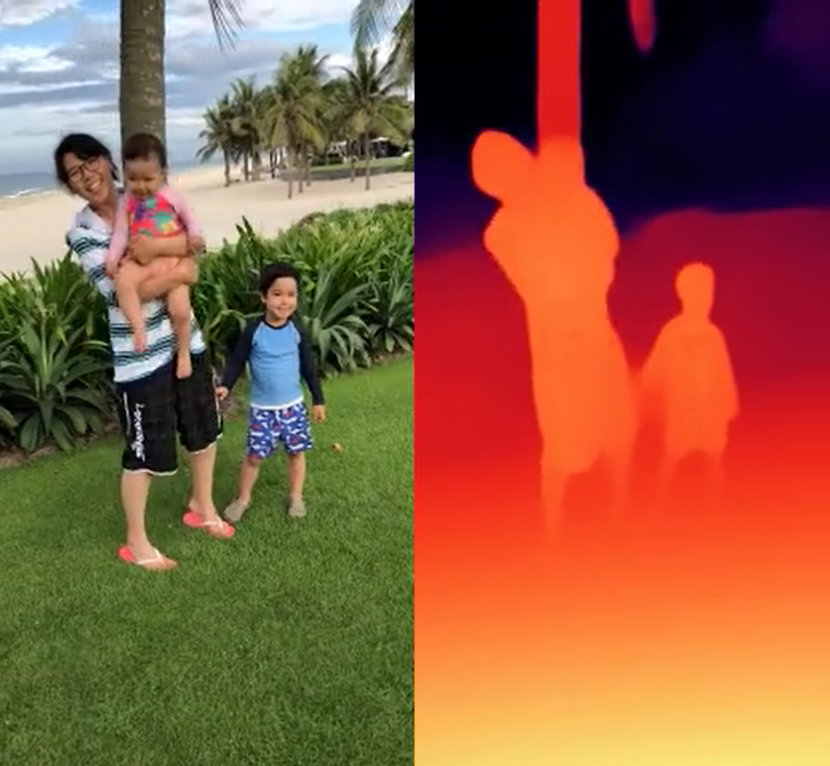
\includegraphics[scale=0.4]{Images/Estado del arte/depthDiferido.png}
    \caption{Ejemplo de mapa de profundidad obtenido en el estudio~\cite{oclusionEnDiferido}.}
    \label{fig:depthDiferido}
\end{figure}